\documentclass[a4paper,twoside]{ctexart}
\usepackage{geometry}
\geometry{margin=1cm,vmargin={0pt,1cm}}
\setlength{\topmargin}{-2cm}
\setlength{\paperheight}{23cm}
\setlength{\paperwidth}{18cm}
\setlength{\textheight}{19.6cm}
\setlength{\textwidth}{15cm}
\usepackage{makecell}
\usepackage{fancyhdr}
\usepackage{siunitx}
\usepackage{amssymb}
\usepackage{indentfirst}
\setlength{\parindent}{0.5em}

\pagenumbering{arabic}

% useful packages.
\usepackage{multirow}
\usepackage{caption}
\usepackage{mathrsfs}
\usepackage{amsfonts}
\usepackage{amsmath}
\usepackage{amsthm}
\usepackage{enumerate}
\usepackage{xcolor,graphicx,float,subfigure}
\usepackage{epstopdf}
\usepackage{multicol}
\usepackage{fancyhdr}
\usepackage{layout}
\usepackage{listings}
\lstset{language=Matlab}
\lstset{breaklines}
\lstset{extendedchars=false}
\usepackage[colorlinks,linkcolor=blue]{hyperref}
\usepackage{xcolor}
\usepackage{cite}
\usepackage[numbers,sort&compress]{natbib} 
\setcitestyle{open={},close={}}
%\usepackage{natbibspacing}
%\renewcommand{\refname}{}
\usepackage{anyfontsize}
%\usepackage[ruled]{algorithm2e}
\usepackage{algorithm}
\usepackage{algorithmicx}
\usepackage{algpseudocode}
\renewcommand{\algorithmicrequire}{\textbf{Input:}}  % Use Input in the format of Algorithm
\renewcommand{\algorithmicensure}{\textbf{Side effect:}} % Use Output in the format of Algorithm


\usepackage{bm}



% some common command
\newcommand{\dif}{\mathrm{d}}
\newcommand{\avg}[1]{\left\langle #1 \right\rangle}
\newcommand{\pdfrac}[2]{\frac{\partial #1}{\partial #2}}
\newcommand{\op}{\odot}
\newcommand{\Eabs}{E_{\mathrm{abs}}}
\newcommand{\Erel}{E_{\mathrm{rel}}}
\newcommand{\Ediv}{\mathrm{div}}%\div是除号
\newcommand{\lrq}[1]{\left( #1 \right)}
\newcommand{\avint}[1]{\frac{1}{\left|#1\right|}\int_{#1}}

\newcommand{\upcite}[1]{\textsuperscript{\textsuperscript{\cite{#1}}}}


\makeatletter
\newcommand\sixteen{\@setfontsize\sixteen{17pt}{6}}
\renewcommand{\maketitle}{\bgroup\setlength{\parindent}{0pt}
\begin{flushleft}
\sixteen\bfseries \@title
\medskip
\end{flushleft}
\textit{\@author}
\egroup}
\makeatother

\CTEXsetup[format={\Large\bfseries}]{section}

\title{曲率流速度场测试}


\begin{document}
\maketitle
\vspace{-3em}
\section{单位圆测例}

以下测试在一个单位圆上均匀取点,并计算由这些示踪点得到的曲率流的速度场。
测试曲线如下:
\begin{equation}
  \left\{
  \begin{array}{l}
    x=\cos{t},\\
    y=\sin{t},\\
    t \in [0,2\pi].
  \end{array}
  \right.
\end{equation}  
测试结果如表\ref{tab:circle1}和\ref{tab:circle2}所示,所用误差范数
$\|\mathrm{E}\|_1$和$\|\mathrm{E}\|_{\infty}$是与精确解之间的网格1-范数
和无穷范数。我们发现结果可以达到相应的收敛阶。

\begin{table}[htbp]
    \centering\begin{tabular}{c|ccccccccc}
        \hline
         &$n=64$&ratio&128&ratio&256&ratio&512&ratio&1024\\
        \hline
        $\|\mathrm{E}\|_1$&5.12e-3&2.01&1.27e-3&2.01&3.17e-4&2.00&7.90e-5&2.00&1.97-5\\
        \hline
        $\|\mathrm{E}\|_{\infty}$&8.03e-4&2.00&2.01e-4&2.00&5.02e-5&2.00&1.26e-5&2.00&3.14e-6\\
        \hline
    \end{tabular}
    \caption{单位圆测例: 误差及收敛阶,$r = 2$}
    \label{tab:circle1}
  \end{table}

  \begin{table}[htbp]
    \centering\begin{tabular}{c|ccccccccc}
        \hline
         &$n=64$&ratio&128&ratio&256&ratio&512&ratio&1024\\
        \hline
        $\|\mathrm{E}\|_1$&4.93e-6&4.01&3.06e-7&4.01&1.91e-8&4.00&1.19e-9&3.79&8.63e-11\\
        \hline
        $\|\mathrm{E}\|_{\infty}$&7.73e-7&4.00&4.84e-8&4.00&3.03e-9&3.93&1.98e-10&1.69&6.13e-11\\
        \hline
    \end{tabular}
    \caption{单位圆测例: 误差及收敛阶,$r = 4$}
    \label{tab:circle2}
  \end{table}

  \section{星型线测例}

以下测试在一个星型曲线上取点,并计算由这些示踪点得到的曲率流的速度场。
测试曲线如下:
\begin{equation}
  \left\{
  \begin{array}{l}
    x=(1+0.3\cos{6t})\cos{t},\\
    y=(1+0.3\cos{6t})\sin{t},\\
    t \in [0,2\pi].
  \end{array}
  \right.
\end{equation}

\begin{figure}[!htp]                                                                       
  \centering                                                                           
  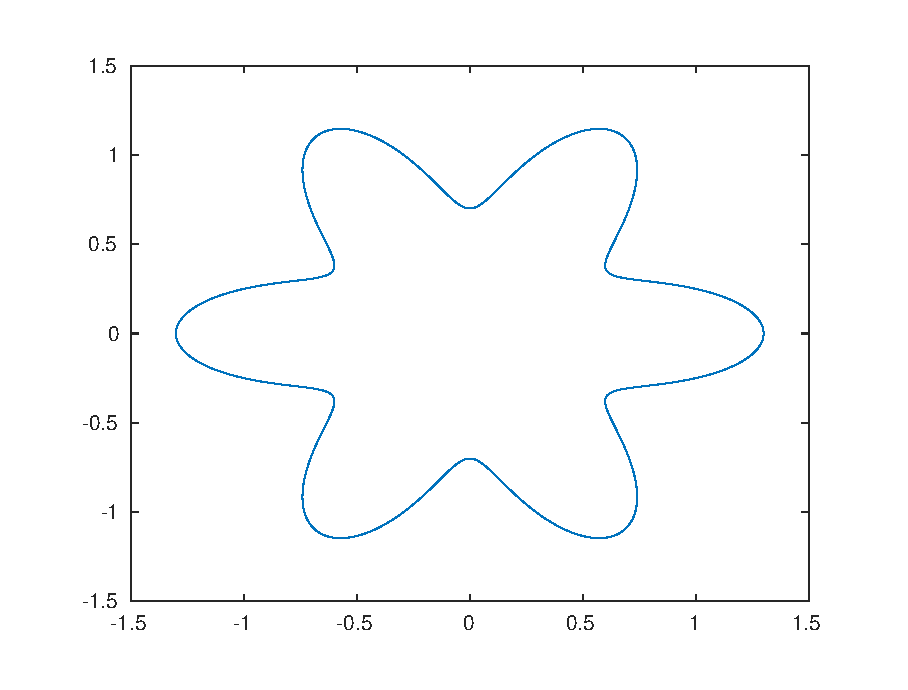
\includegraphics[width=8cm]{star.eps}                                           
  \caption{星型线}                        
\end{figure}

\newpage 测试结果如表\ref{tab:star1}和\ref{tab:star2}所示,所用误差范数
$\|\mathrm{E}\|_1$和$\|\mathrm{E}\|_{\infty}$是与参考解之间的网格1-范数
和无穷范数,参考解是对示踪点列进一步加密的结果。我们发现结果可以达到相应的收敛阶。

\begin{table}[htbp]
    \centering\begin{tabular}{c|ccccccc}
        \hline
         &$n=256$&ratio&512&ratio&1024&ratio&2048\\
        \hline
        $\|\mathrm{E}\|_1$&2.10e-1&1.99&5.29e-02&2.02&1.30e-2&2.07&3.11e-3\\
        \hline
        $\|\mathrm{E}\|_{\infty}$&1.02e+0&1.93&2.68e-1&2.00&6.71e-2&2.07&1.60e-2\\
        \hline
    \end{tabular}
    \caption{星型线测例: 误差及收敛阶,$r = 2$}
    \label{tab:star1}
  \end{table}

  \begin{table}[htbp]
    \centering\begin{tabular}{c|ccccccc}
        \hline
         &$n=256$&ratio&512&ratio&1024&ratio&2048\\
        \hline
        $\|\mathrm{E}\|_1$&5.83e-2&3.78&4.24e-3&3.96&2.72e-4&4.00&1.70e-5\\
        \hline
        $\|\mathrm{E}\|_{\infty}$&3.27e-1&3.53&2.82e-2&3.89&1.91e-3&3.98&1.21e-4\\
        \hline
    \end{tabular}
    \caption{星型线测例: 误差及收敛阶,$r = 4$}
    \label{tab:star2}
\end{table}







\end{document}
